\subsection{Кеплеровы элементы орбиты}

\textbf{Кеплеровы элементы} --- шесть элементов орбиты, определяющие положение небесного тела в пространстве в задаче двух тел:
\begin{enumerate}
\item Большая полулось($a$);
\item Эксцентриситет ($e$);
\item Наклонение($i$);
\item Аргумент перицентра($\omega$);
\item Долгота восходящего узла($\Omega$);
\item Средняя аномалия ($M_0$);
\end{enumerate}
Первые два определяют форму орбиты, третий, четвёртый и пятый — ориентацию плоскости орбиты по отношению к базовой системе координат, шестой — положение тела на орбите (Рис.5).

\textbf{Наклонение} --- небесного тела — это угол между плоскостью его орбиты и плоскостью эклиптики.
\textbf{Аргумент перицентра} --- угол между направлениями из притягивающего центра на восходящий узел орбиты и на перицентр.

\textbf{Долгота восходящего узла} --- угол в плоскости эклиптики между направлением на точку весеннего равноденствия и восходящий узел орбиты. Отсчитывается против часовой стрелки от направления на точку весеннего равноденствия.

\textbf{Средняя аномалия} для тела, движущегося по невозмущённой орбите --- произведение его среднего движения и интервала времени после прохождения перицентра.

\textbf{Узлы орбиты} --- точки пересечения орбиты и плоскости эклиптики.

\textbf{Восходящий узел} --- точка, в которой тело пересекает плоскость эклиптики при движении в северноим направлении, а \textbf{нисходящий} --- в южном.

\textbf{Истинная аномалия ($\nu$)} --- угол между радиус вектором и направлением на перицентр.
\begin{center}
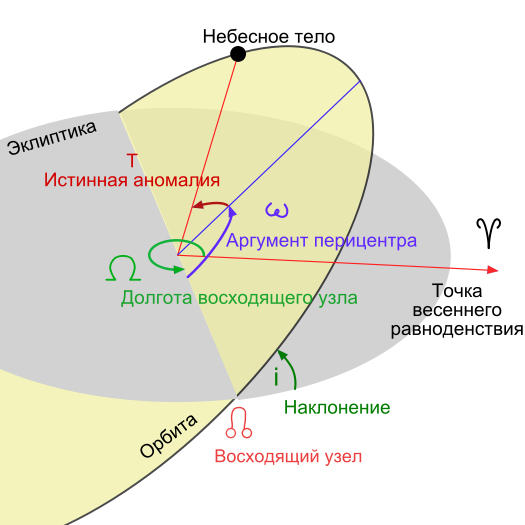
\includegraphics[scale=0.31]{Orbit-elem}
\begin{figure}[h!]
\caption{Кеплеровы элементы орбиты}
\end{figure}
\end{center}